\documentclass{article}
\usepackage{tikz,amsmath,siunitx}
\usepackage{pgfplots}
\usepackage{listings}
\usetikzlibrary{arrows,snakes,backgrounds,patterns,matrix,shapes,fit,calc,shadows,plotmarks}
%\usepackage[graphics,tightpage,active]{preview}
%\PreviewEnvironment{tikzpicture}
%\PreviewEnvironment{equation}
%\PreviewEnvironment{equation*}
\title{CS540 Practice Assignment 5}
\author{Dustin Ingram, Aaron Rosenfeld, Tom Wambold}
\newlength{\imagewidth}
\newlength{\imagescale}
\pagestyle{empty}
\thispagestyle{empty}
\lstset{breaklines=true}
\begin{document}
\maketitle
\newpage
\section{Tasks}
\begin{enumerate}
    \item Determine machine parameters (CPU type, CPU speed, CPU info such as pipeline and functional units, memory, cache info)
    \item Time and instrument matrix multiplication code.
    \item Experiment with variants of matrix multiplication.
    \item Install ATLAS and MKL (compare to Numeric Recipes)
\end{enumerate}
\newpage
\section{Results}
\subsection{System \& Kernel Information}
\begin{lstlisting}
$ uname -a
Linux float.cs.drexel.edu 2.6.35-28-generic #50-Ubuntu SMP Fri Mar 18 18:42:20 UTC 2011 x86_64 GNU/Linux
\end{lstlisting}
\subsection{GCC Version Information}
\begin{lstlisting}
$ gcc --version
gcc (Ubuntu/Linaro 4.4.4-14ubuntu5) 4.4.5
\end{lstlisting}
\subsection{CPU Information}
\begin{lstlisting}
$ cat /proc/cpuinfo
processor	: 15
vendor_id	: GenuineIntel
cpu family	: 6
model		: 44
model name	: Intel(R) Xeon(R) CPU           L5630  @ 2.13GHz
stepping	: 2
cpu MHz		: 1600.000
cache size	: 12288 KB
physical id	: 1
siblings	: 8
core id		: 10
cpu cores	: 4
apicid		: 53
initial apicid	: 53
fpu		: yes
fpu_exception	: yes
cpuid level	: 11
wp		: yes
flags		: fpu vme de pse tsc msr pae mce cx8 apic sep mtrr pge mca cmov pat pse36 clflush dts acpi mmx fxsr sse sse2 ss ht tm pbe syscall nx pdpe1gb rdtscp lm constant_tsc arch_perfmon pebs bts rep_good xtopology nonstop_tsc aperfmperf pni pclmulqdq dtes64 monitor ds_cpl vmx smx est tm2 ssse3 cx16 xtpr pdcm dca sse4_1 sse4_2 popcnt aes lahf_lm ida arat dts tpr_shadow vnmi flexpriority ept vpid
bogomips	: 4266.84
clflush size	: 64
cache_alignment	: 64
address sizes	: 40 bits physical, 48 bits virtual
power management:
\end{lstlisting}
\subsection{Memory Information}
\begin{lstlisting}
$ papi_mem_info
Memory Cache and TLB Hierarchy Information.
------------------------------------------------------------------------
TLB Information.
  There may be multiple descriptors for each level of TLB
  if multiple page sizes are supported.

L1 Instruction TLB:
  Page Size:           2048 KB
  Number of Entries:      7
  Associativity:       Full

L1 Instruction TLB:
  Page Size:           4096 KB
  Number of Entries:      7
  Associativity:       Full

L1 Data TLB:
  Page Size:              4 KB
  Number of Entries:     64
  Associativity:          4

L1 Data TLB:
  Page Size:           2048 KB
  Number of Entries:     32
  Associativity:          4

L1 Data TLB:
  Page Size:           4096 KB
  Number of Entries:     32
  Associativity:          4

L1 Instruction TLB:
  Page Size:              4 KB
  Number of Entries:     64
  Associativity:          4


Cache Information.

L1 Data Cache:
  Total size:            32 KB
  Line size:             64 B
  Number of Lines:      512
  Associativity:          8

L1 Instruction Cache:
  Total size:            32 KB
  Line size:             64 B
  Number of Lines:      512
  Associativity:          4

L2 Unified Cache:
  Total size:           256 KB
  Line size:             64 B
  Number of Lines:     4096
  Associativity:          8

L3 Unified Cache:
  Total size:         12288 KB
  Line size:             64 B
  Number of Lines:   196608
  Associativity:         16

mem_info.c                               PASSED
\end{lstlisting}
\subsection{Timing of Matrix Multiplication Code}
\pgfplotsset{width=\textwidth,compat=1.4}
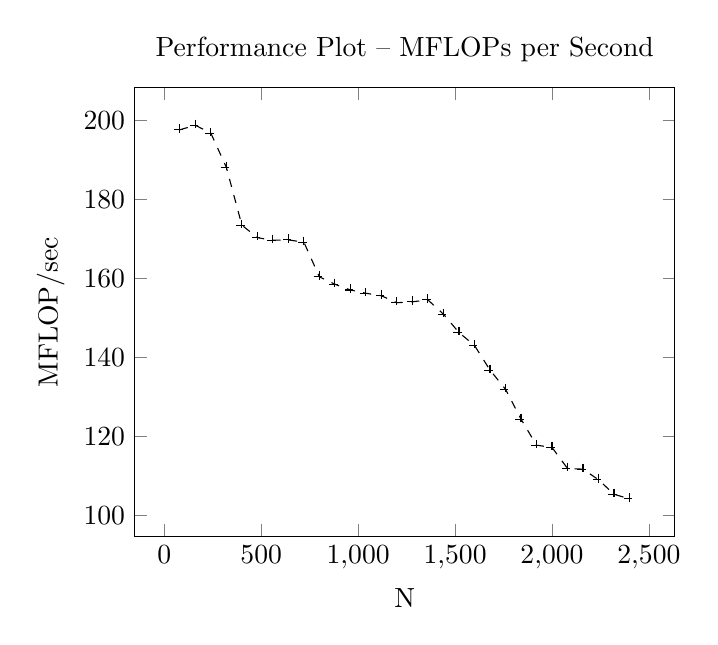
\begin{tikzpicture}
\begin{axis}[
xlabel=N,
ylabel=MFLOP/sec,
legend pos=north east,
title=Performance Plot -- MFLOPs per Second] 

\addplot[color=black,mark=+,dashed] coordinates {
(	80	,	197.6929826255	)
(	160	,	198.8440728155	)
(	240	,	196.8224896797	)
(	320	,	188.1825815155	)
(	400	,	173.5493932539	)
(	480	,	170.3740100077	)
(	560	,	169.7130381458	)
(	640	,	169.8101313916	)
(	720	,	169.2183857305	)
(	800	,	160.4442840376	)
(	880	,	158.5767076941	)
(	960	,	157.1294912172	)
(	1040	,	156.300815689	)
(	1120	,	155.6551119783	)
(	1200	,	153.8961007297	)
(	1280	,	154.1316348082	)
(	1360	,	154.6040968069	)
(	1440	,	150.9996898904	)
(	1520	,	146.3545865429	)
(	1600	,	143.0928800391	)
(	1680	,	136.8428730177	)
(	1760	,	132.0082614054	)
(	1840	,	124.4330371376	)
(	1920	,	117.8187102184	)
(	2000	,	117.2567412855	)
(	2080	,	111.9249619669	)
(	2160	,	111.7427307871	)
(	2240	,	109.0673289854	)
(	2320	,	105.3859142508	)
(	2400	,	104.2266883241	)
};
\end{axis}
\end{tikzpicture}
\subsection{Comparison with ATLAS and MKL}
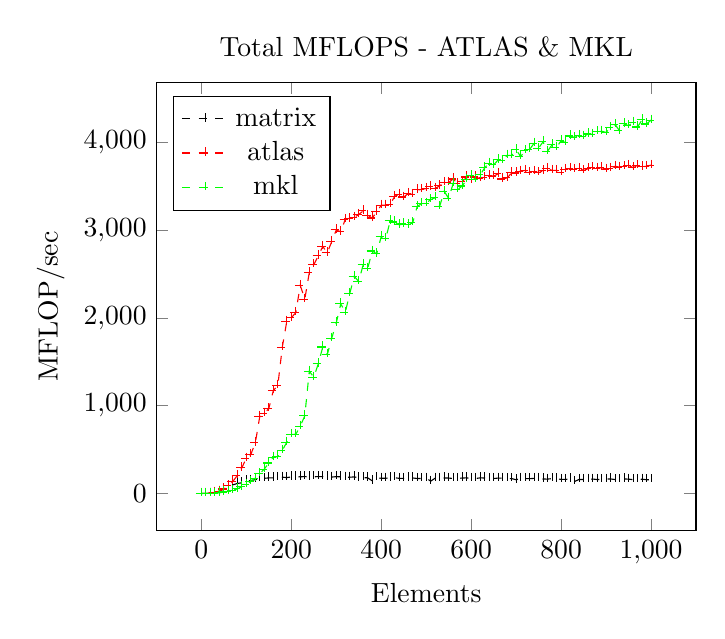
\begin{tikzpicture}
\begin{axis}[
xlabel=Elements,
ylabel=MFLOP/sec,
legend pos=north west,
title=Total MFLOPS - ATLAS \& MKL] 
\legend{matrix, atlas, mkl}

\addplot[color=black,mark=|,dashed] coordinates {
(	0	,	0	)
(	10	,	0.4	)
(	20	,	3.2032	)
(	30	,	10.8046	)
(	40	,	25.6058	)
(	50	,	50.0134	)
(	60	,	72.0156666667	)
(	70	,	98.0095714286	)
(	80	,	113.7843333333	)
(	90	,	121.505	)
(	100	,	142.8632857143	)
(	110	,	147.9002222222	)
(	120	,	157.0971818182	)
(	130	,	169.0094230769	)
(	140	,	171.5079375	)
(	150	,	177.6393421053	)
(	160	,	178.0924130435	)
(	170	,	181.9679074074	)
(	180	,	185.1525714286	)
(	190	,	180.5226973684	)
(	200	,	188.2455647059	)
(	210	,	187.1105454545	)
(	220	,	190.1528303571	)
(	230	,	191.6205748032	)
(	240	,	189.4197054795	)
(	250	,	190.5972073171	)
(	260	,	191.061673913	)
(	270	,	192.0659902439	)
(	280	,	187.7087692308	)
(	290	,	186.2717061069	)
(	300	,	191.5337411348	)
(	310	,	189.1888349206	)
(	320	,	185.2011525424	)
(	330	,	184.8618766067	)
(	340	,	188.5442182254	)
(	350	,	178.0678755187	)
(	360	,	179.5666365385	)
(	370	,	177.8448438597	)
(	380	,	143.6029856209	)
(	390	,	179.0752126697	)
(	400	,	172.8597044534	)
(	410	,	173.0803613551	)
(	420	,	178.4448002407	)
(	430	,	179.8023062147	)
(	440	,	171.6883575025	)
(	450	,	171.2397295775	)
(	460	,	178.3815934066	)
(	470	,	176.0768033898	)
(	480	,	170.2394238462	)
(	490	,	169.7333561644	)
(	500	,	174.8028357792	)
(	510	,	140.2505951374	)
(	520	,	174.0180265925	)
(	530	,	173.1182736781	)
(	540	,	176.2407276286	)
(	550	,	175.2522636842	)
(	560	,	169.8761527308	)
(	570	,	169.9447276479	)
(	580	,	175.6675276653	)
(	590	,	177.3352502157	)
(	600	,	169.9503871855	)
(	610	,	170.224885725	)
(	620	,	177.6099143708	)
(	630	,	175.7442166433	)
(	640	,	169.8663486565	)
(	650	,	169.9349366306	)
(	660	,	175.3394981718	)
(	670	,	175.1706802444	)
(	680	,	169.5425076757	)
(	690	,	169.3432868177	)
(	700	,	155.8504488082	)
(	710	,	175.0731199902	)
(	720	,	169.2176910532	)
(	730	,	167.97202761	)
(	740	,	172.1009085702	)
(	750	,	173.1877699405	)
(	760	,	164.4974278495	)
(	770	,	163.4961207297	)
(	780	,	169.4885009809	)
(	790	,	167.064037225	)
(	800	,	160.3215160281	)
(	810	,	159.7922644144	)
(	820	,	165.3097526576	)
(	830	,	136.382618327	)
(	840	,	159.2488376275	)
(	850	,	159.0740377749	)
(	860	,	163.5848219424	)
(	870	,	163.9590854265	)
(	880	,	158.6312360191	)
(	890	,	158.2897463272	)
(	900	,	163.7367694638	)
(	910	,	164.992402187	)
(	920	,	158.3649005486	)
(	930	,	157.8114530576	)
(	940	,	164.9135778042	)
(	950	,	163.1584571293	)
(	960	,	157.0377796595	)
(	970	,	156.5451090738	)
(	980	,	162.4772825974	)
(	990	,	156.4535901547	)
(	1000	,	156.5736698217	)
};

\addplot[color=red,mark=+,dashed] coordinates {
(	0	,	0	)
(	10	,	0.4268333333	)
(	20	,	2.808	)
(	30	,	9.3195	)
(	40	,	26.5624	)
(	50	,	50.719	)
(	60	,	86.4434	)
(	70	,	137.324	)
(	80	,	205.1048	)
(	90	,	292.1822	)
(	100	,	400.891	)
(	110	,	444.7231666667	)
(	120	,	576.1273333333	)
(	130	,	879.1894	)
(	140	,	915.2995	)
(	150	,	965.0721428571	)
(	160	,	1171.4992857143	)
(	170	,	1228.401625	)
(	180	,	1666.5668571429	)
(	190	,	1960.4772857143	)
(	200	,	2000.8075	)
(	210	,	2058.9981111111	)
(	220	,	2367.9025555556	)
(	230	,	2212.3821818182	)
(	240	,	2513.8977272727	)
(	250	,	2604.8005833333	)
(	260	,	2704.7863846154	)
(	270	,	2812.9822142857	)
(	280	,	2739.286375	)
(	290	,	2869.6467647059	)
(	300	,	3000.5403888889	)
(	310	,	2979.67925	)
(	320	,	3121.6697619048	)
(	330	,	3125.8846086957	)
(	340	,	3144.6282	)
(	350	,	3176.1897037037	)
(	360	,	3218.0882068966	)
(	370	,	3166.43125	)
(	380	,	3136.2219142857	)
(	390	,	3207.2087567568	)
(	400	,	3282.2656666667	)
(	410	,	3282.2690476191	)
(	420	,	3293.2951555556	)
(	430	,	3383.7626170213	)
(	440	,	3408.02926	)
(	450	,	3375.1879074074	)
(	460	,	3415.4921052632	)
(	470	,	3404.4599836066	)
(	480	,	3456.379734375	)
(	490	,	3460.6927647059	)
(	500	,	3472.8944861111	)
(	510	,	3491.0184736842	)
(	520	,	3472.0883827161	)
(	530	,	3503.335682353	)
(	540	,	3538.8854382023	)
(	550	,	3540.3917872341	)
(	560	,	3580.9580306123	)
(	570	,	3527.7510476191	)
(	580	,	3547.8122818182	)
(	590	,	3603.4613684211	)
(	600	,	3570.7332809917	)
(	610	,	3603.3144603175	)
(	620	,	3584.103037594	)
(	630	,	3597.9989280576	)
(	640	,	3616.0676482759	)
(	650	,	3613.8563355263	)
(	660	,	3639.5752594937	)
(	670	,	3580.91075	)
(	680	,	3593.5894457143	)
(	690	,	3650.1957388889	)
(	700	,	3649.1290053192	)
(	710	,	3671.0754564103	)
(	720	,	3677.5683891626	)
(	730	,	3652.8371643193	)
(	740	,	3667.2599140272	)
(	750	,	3652.7844935065	)
(	760	,	3673.593874477	)
(	770	,	3696.809708502	)
(	780	,	3679.0136395349	)
(	790	,	3679.4631231343	)
(	800	,	3657.2796321429	)
(	810	,	3690.6784618056	)
(	820	,	3700.600818792	)
(	830	,	3689.1831129032	)
(	840	,	3702.242684375	)
(	850	,	3677.5161467066	)
(	860	,	3698.1280755814	)
(	870	,	3709.9912478873	)
(	880	,	3703.8823722826	)
(	890	,	3710.5589131579	)
(	900	,	3691.2531063291	)
(	910	,	3703.1382923833	)
(	920	,	3725.8670550239	)
(	930	,	3715.4587759815	)
(	940	,	3724.7757914798	)
(	950	,	3736.030540305	)
(	960	,	3709.6667924528	)
(	970	,	3732.8977873211	)
(	980	,	3720.2723339921	)
(	990	,	3724.8945758157	)
(	1000	,	3738.4754093458	)
};

\addplot[color=green,mark=+,dashed] coordinates {
(	0	,	0.0006	)
(	10	,	0.217	)
(	20	,	0.8768	)
(	30	,	3.1092	)
(	40	,	6.6482	)
(	50	,	16.8805	)
(	60	,	22.1326	)
(	70	,	36.2232	)
(	80	,	52.1888	)
(	90	,	76.1296	)
(	100	,	101.6606	)
(	110	,	137.9136	)
(	120	,	175.3476	)
(	130	,	226.3708	)
(	140	,	277.6574	)
(	150	,	346.3906	)
(	160	,	414.0528	)
(	170	,	418.9753333333	)
(	180	,	490.5525	)
(	190	,	583.431	)
(	200	,	672.4343333333	)
(	210	,	673.989	)
(	220	,	766.543	)
(	230	,	884.0058571429	)
(	240	,	1392.9092	)
(	250	,	1323.2058333333	)
(	260	,	1476.6396666667	)
(	270	,	1667.7031666667	)
(	280	,	1580.098	)
(	290	,	1769.3367142857	)
(	300	,	1942.3812857143	)
(	310	,	2158.9104285714	)
(	320	,	2061.921125	)
(	330	,	2277.227125	)
(	340	,	2472.641875	)
(	350	,	2412.9931111111	)
(	360	,	2608.5525555556	)
(	370	,	2563.845	)
(	380	,	2760.3272	)
(	390	,	2727.83	)
(	400	,	2926.3251818182	)
(	410	,	2904.4681666667	)
(	420	,	3104.1189166667	)
(	430	,	3090.857	)
(	440	,	3058.5465714286	)
(	450	,	3068.6757333333	)
(	460	,	3057.5343125	)
(	470	,	3083.2912352941	)
(	480	,	3269.1392941177	)
(	490	,	3299.5425	)
(	500	,	3305.3149473684	)
(	510	,	3346.6256	)
(	520	,	3367.4134285714	)
(	530	,	3269.8049130435	)
(	540	,	3441.6206956522	)
(	550	,	3359.16796	)
(	560	,	3530.53256	)
(	570	,	3461.0877777778	)
(	580	,	3501.2814285714	)
(	590	,	3572.422	)
(	600	,	3617.1212333333	)
(	610	,	3577.1946875	)
(	620	,	3627.5747272727	)
(	630	,	3707.5892352941	)
(	640	,	3761.5400571429	)
(	650	,	3740.9967567568	)
(	660	,	3798.8669210526	)
(	670	,	3788.627	)
(	680	,	3850.7983902439	)
(	690	,	3848.8511395349	)
(	700	,	3913.3310454546	)
(	710	,	3835.4243617021	)
(	720	,	3903.1701875	)
(	730	,	3917.99446	)
(	740	,	3987.647	)
(	750	,	3932.9590740741	)
(	760	,	4005.3228545455	)
(	770	,	3898.3136949153	)
(	780	,	3971.8061166667	)
(	790	,	3941.725015873	)
(	800	,	4017.000421875	)
(	810	,	3994.2571641791	)
(	820	,	4070.8447205882	)
(	830	,	4054.5810985916	)
(	840	,	4075.8074246575	)
(	850	,	4067.8263026316	)
(	860	,	4093.1910641026	)
(	870	,	4091.6738888889	)
(	880	,	4120.9979759036	)
(	890	,	4125.1024534884	)
(	900	,	4110.7215505618	)
(	910	,	4166.5750879121	)
(	920	,	4201.7198494624	)
(	930	,	4129.2770510204	)
(	940	,	4209.8284747475	)
(	950	,	4187.2930970874	)
(	960	,	4227.9567619048	)
(	970	,	4173.2397636364	)
(	980	,	4254.085963964	)
(	990	,	4206.6146896552	)
(	1000	,	4251.7935847458	)
};

\end{axis}
\end{tikzpicture}


\end{document}
